\documentclass[12pt,letterpaper]{article}


\newcommand{\doctitle}{Scientific Computing Homework 2}
\newcommand{\docauthor}{Matthew Duschenes}
\newcommand{\docaffil}{Department of Applied Physics, University of Michigan}
\newcommand{\docheader}{NERS 570 \ - Homework 2 - \docauthor}
\newcommand{\docfooter}{\docaffil}


% Margins
\usepackage[margin=0.75in,marginparsep=0pt,paperwidth=216mm,paperheight=279mm]{geometry}

% Headers
\usepackage{fancyhdr}
\geometry{headheight=15pt}
\renewcommand{\headrulewidth}{0.4pt}% default is 0.4pt
\renewcommand{\footrulewidth}{0.4pt}% default is 0pt
\geometry{headheight=15pt}
\geometry{headsep=10pt}
\setlength{\skip\footins}{10pt} % gap between text and footer
\fancyhf{}
\fancyhead[R]{\docheader}
\fancyfoot[LE,RO]{\thepage}
\fancyfoot[LO,RE]{\docfooter}

% \makeatletter
% \if@twoside
% \fancyfoot[LE,RO]{\thepage}
% \fancyfoot[LO,RE]{\docfooter}
% \else
% \fancyfoot[R]{\thepage}
% \fancyfoot[L]{\docfooter}
% \fi
% \makeatother
% \fancyhead[R]{\docheader}


% Title
\usepackage{titling}
% \usepackage[affil-it]{authblk}
\usepackage[nodayofweek]{datetime}
\usepackage[super]{nth}

% \newdateformat{monthdayyear}{%
%   \monthname[\THEMONTH]~\THEDAY,~ \THEYEAR}
% \newdateformat{mydate}{\monthname[\THEMONTH] \nth[\THEDAY], \THEYEAR}


% Make Title
\pagestyle{fancy}
% \renewcommand*{\Authfont}{\bfseries}
% \renewcommand*{\Affilfont}{\normalfont\itshape}
\pretitle{\begin{center}\vskip -50pt}%
\title{\large \doctitle}
\posttitle{\end{center}}
\preauthor{\begin{center} \vskip -20pt}
\author{}
\postauthor{\end{center} \vskip -20pt}
\predate{\begin{center} \vskip -20pt}
\date{}%\small{\today}}
\postdate{\end{center} \vskip -20pt}% -42.5pt


% Fonts
\usepackage[singlespacing]{setspace}

 
% Math
\usepackage{amsmath}
\usepackage{amssymb}
\usepackage{physics}


% Figures
\usepackage{floatrow}
\usepackage{multicol}
\usepackage{grffile}
\usepackage{caption}
\usepackage{subcaption}
\usepackage{graphicx,xcolor}
\PassOptionsToPackage{export}{adjustbox}

% HypperReferences
\usepackage[pdftex,draft=false]{hyperref}
\hypersetup{
    colorlinks=true,
    linkcolor=black,
    citecolor=black,
    urlcolor=black}
\usepackage{url}

% References
\usepackage[capitalize]{cleveref}


% Code
\usepackage{minted}
\renewcommand\listingscaption{Code}
\floatsetup[listing]{style=Plaintop}    

\crefname{listing}{Code.}{Code}
\newminted{python}{frame=lines,framerule=2pt,float=ht}
\setminted{breaklines,frame=single,framesep=2pt,breakindent=10pt,breakafter={,},breaksymbolleft=}

\newenvironment{longlisting}{\captionsetup{type=listing}}{}
\newcommand{\code}[4]{
% \begin{listing}[ht]
\begin{longlisting}
    \caption{#3}
    \inputminted{#1}{#2}
    \label{code:#4}
\end{longlisting}
% \end{listing}
}


 % Commands
\newcommand{\reals}{\mathbb{R}}
\DeclareMathOperator*{\argmax}{arg\,max}
\DeclareMathOperator*{\argmin}{arg\,min}

\newcommand{\eqtxt}[1]{\overset{#1}=}
\newcommand{\repo}[2]{\href{https://github.com/bkochuna/ners570f20-Lab06/#1/#2}{\##2}}


%%%%%%%%%%%%%%%%%%%%%%%%%%%%%%%%%%%%%%%%%%%%%%%%%%%
\begin{document}
\maketitle
\thispagestyle{fancy}
\singlespacing
%%%%%%%%%%%%%%%%%%%%%%%%%%%%%%%%%%%%%%%%%%%%%%%%

\section{Spectral Radius of Fixed Point Methods}
Fixed Point iterative methods involve finding the solutions to 
\begin{equation}
  Ax = b  
\end{equation}
by decomposing the matrix into a form such that iterations are
\begin{equation}
  x_{n+1} = Bx_{n} + c,  
\end{equation}
where $B$ is matrix that is typically a function of $A$, and $c$ is a function of $A$ and $b$. These iteration matrices are generally most easily expressed when $A$ is decomposed as its diagonal, lower, and upper triangular components:
\begin{equation}
  A = D + L + U,
\end{equation} 
since the forms of these matrices make them easily invertible for use in the iterative updates to $x$.

Given an initial guess $x_0$ the error $e_{n} = x_{n} - x$ is
\begin{equation}
  e_n = B^{n}e_0, 
\end{equation}
and the relative norm of the error is:
\begin{equation}
  \frac{\norm{e_{n}}}{\norm{e_{0}}} \leq \norm{B^n}.
\end{equation} 

This norm of $\norm{B^n}$ can be approximated by upper bounds, and in the case of the 2-norm, in terms of the spectral radius $\rho(B)$:
\begin{equation}
  \norm{B^n} \leq \norm{B}^n \leq \rho(B)^n.
\end{equation}
Therefore the spectral radius of $B$ can be found from either directly calculating (through some other iterative method using a numerical library) for the eigenvalues of $B$, or from measuring the norms of the residual over the iterations, with the last iteration likely giving the best estimate for the spectral radius:

\begin{equation}
  \rho(B) = \max_{\lambda} \abs{\lambda(B)} = {\left(\frac{\norm{e_{n}}}{\norm{e_{0}}}\right)}^{1/n}.
\end{equation}


The condition number of $A$ is defined in the 2-norm, and can be defined,
\begin{equation}
  \kappa(A) = \norm{A}\norm{A^{-1}} = \frac{\sigma_{\textrm{max}}}{\sigma_{\textrm{min}}} \eqtxt{A^TA=AA^T} \frac{\lambda_{\textrm{max}}}{\lambda_{\textrm{min}}},
\end{equation}
where $\sigma$ are the singular values of $A$, and the last equality for eigenvalues is solely when $A$ is normal.


\subsection{Jacobi Method}
For the Jacobi method, the iterations proceed such that
\begin{align}
  B &= -D^{-1}(L+U) \\
  c &= D^{-1}b.
\end{align}



\subsection{Gauss-Seidel Method}
For the Gauss-Seidel method, the iterations proceed such that
\begin{align}
  B &= -(D+L)^{-1}U \\
  c &= (D+L)^{-1}b.
\end{align}


\subsection{Fixed Point Iteration Results}
As shown in \cref{fig:FixedPt}, the numerical and analytic results somewhat agree, due to the analytic result of the relative error being an upper bound, and so the analytic spectral radius will generally be larger than the estimate from numerical error of the iterative method. In general, for both the Jacobi and Gauss-Seidel methods, the numerical and analytic methods roughly agree, converging to $\rho \to 1$ (from other analytic analysis).

In general, the spectral radius $\rho(B)$ is smaller for the \textbf{Gauss-Seidel} method. This is assumed to be because this method can be shown to converge polynomially faster than the Jacobi method, leading to the error, scaling as $\rho^n$, decreasing faster if the spectral radius is smaller.


When the condition number is calculated for $A$, it is seen that due to the condition number being proportional to the reciprocal of the minimum eigenvalue, and that eigenvalue $\lambda_{\textrm{min}} \to 0$ as the grid size approaches infinity, the condition number will grow without bound. 


\begin{figure}[H]
  \centering
  %  trim={<left> <lower> <right> <upper>}
  % \captionsetup{skip=-12pt,format=hang}
  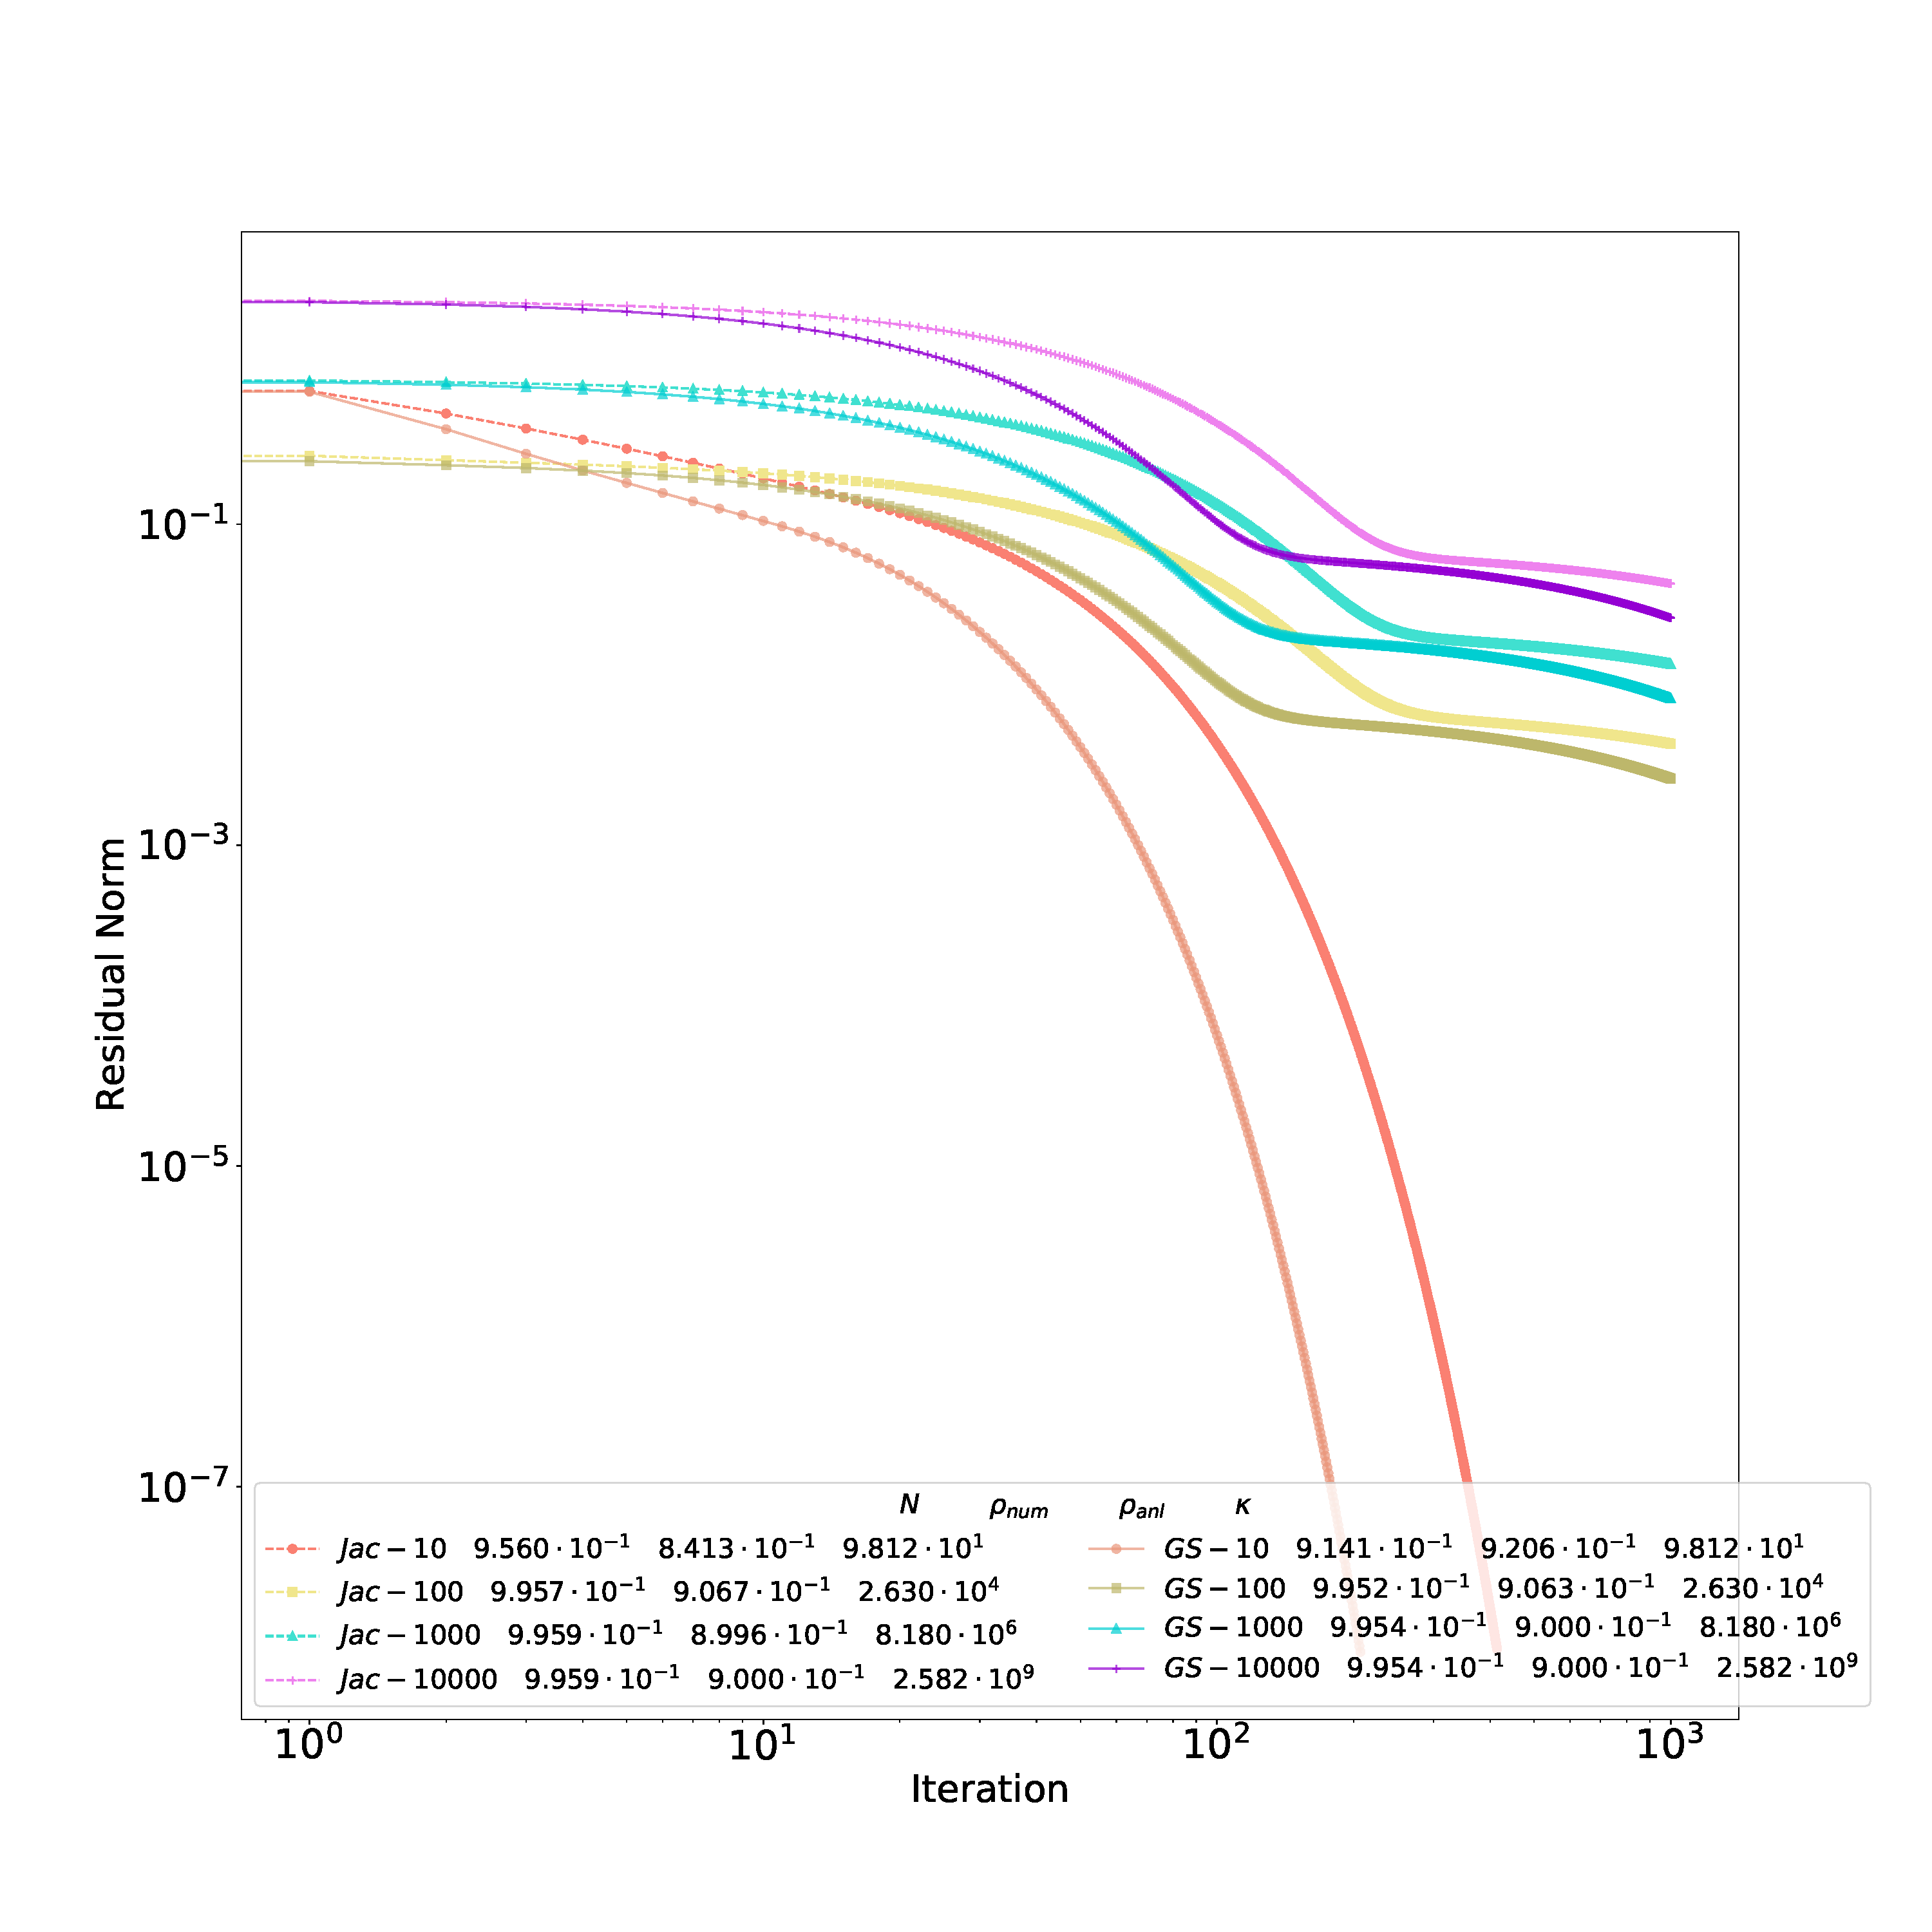
\includegraphics[width=\textwidth]{figures/Ex1.pdf}
  % \vspace{-8pt}
  \caption{Residual norms over iterations for $d=1$ Laplace's equation, using Jacobi and Gauss-Seidel methods. Shown in the legend are eigenvalue statistics for various grid sizes.}
  \label{fig:FixedPt}
\end{figure}

Please refer to the code in \cref{code:Ex1} the Appendix that produces these results.



\newpage
\section{QR Factorization}
In order to perform the QR factorization, the following \textit{QR},class in \cref{code:QR} was used. The QR algorithm uses the modified Graham-Schmidt algorithm, which orthogonalizes a basis for $A$ by removing parallel components from later column vectors for $A$, before they are transformed into their basis counterpart.

The matrix to be factored is the $2\times d$-pt stencil for the Laplacian, for $d=2$ dimensions, with Dirichlet (non-periodic) boundary conditions, for a system with length along each dimension $n$. Here, the central position $x_{ij}$ is multiplied by $2d$, and subtracted from it are the nearest neighbors in the Cartesian grid, which are some permutations of $\pm 1, \pm q*n$, some multiple of $n$. This construction of the matrix, and results are from \cref{code:PDE}.

The code is compiled from the Makefile in \cref{code:make}, and when run <n> is called, the resulting QR algorithm output is shown in \cref{code:QRout}. The output includes printouts for $n=4$, and shows the matrices $A$, $Q$, $R$, as well as the orthonormality of the column vectors $q_i$ of $Q$, and the product of the $QR$ matrices, yielding back $A$ (within $10^{-15}$).

\code{python}{figures/pde.txt}{QR factorization output}{QRout}



\newpage
\section{UML Diagrams}

\subsection{Sequence Diagram for PETSc Ex15}
For this sequence diagram in \cref{fig:ex15}, the ex15 has a fairly linear sequence of processes, where:
\begin{enumerate}
  \item Declare variables, including solution vectors, the linear system matrix, the solver type, and the preconditioner type.
  \item Read in user inputs and with default settings, initialize variable values.
  \item Create vectors and matrix using PETSc parallelism and assemble.
  \item Start linear algebra solver, calls to MatMult for initial rhs solution
  \item Calls to KSPCreate, KSPSetOperators, KSPGetPC, PCSetup
  \item Solve linear system with KSPSolve
  \item Check error with VecNorm,KSPGetIterationNumber
  \item Destroy objects (ksp,u,b)
\end{enumerate}
\begin{figure}[H]
  \centering
  %  trim={<left> <lower> <right> <upper>}
  % \captionsetup{skip=-12pt,format=hang}
  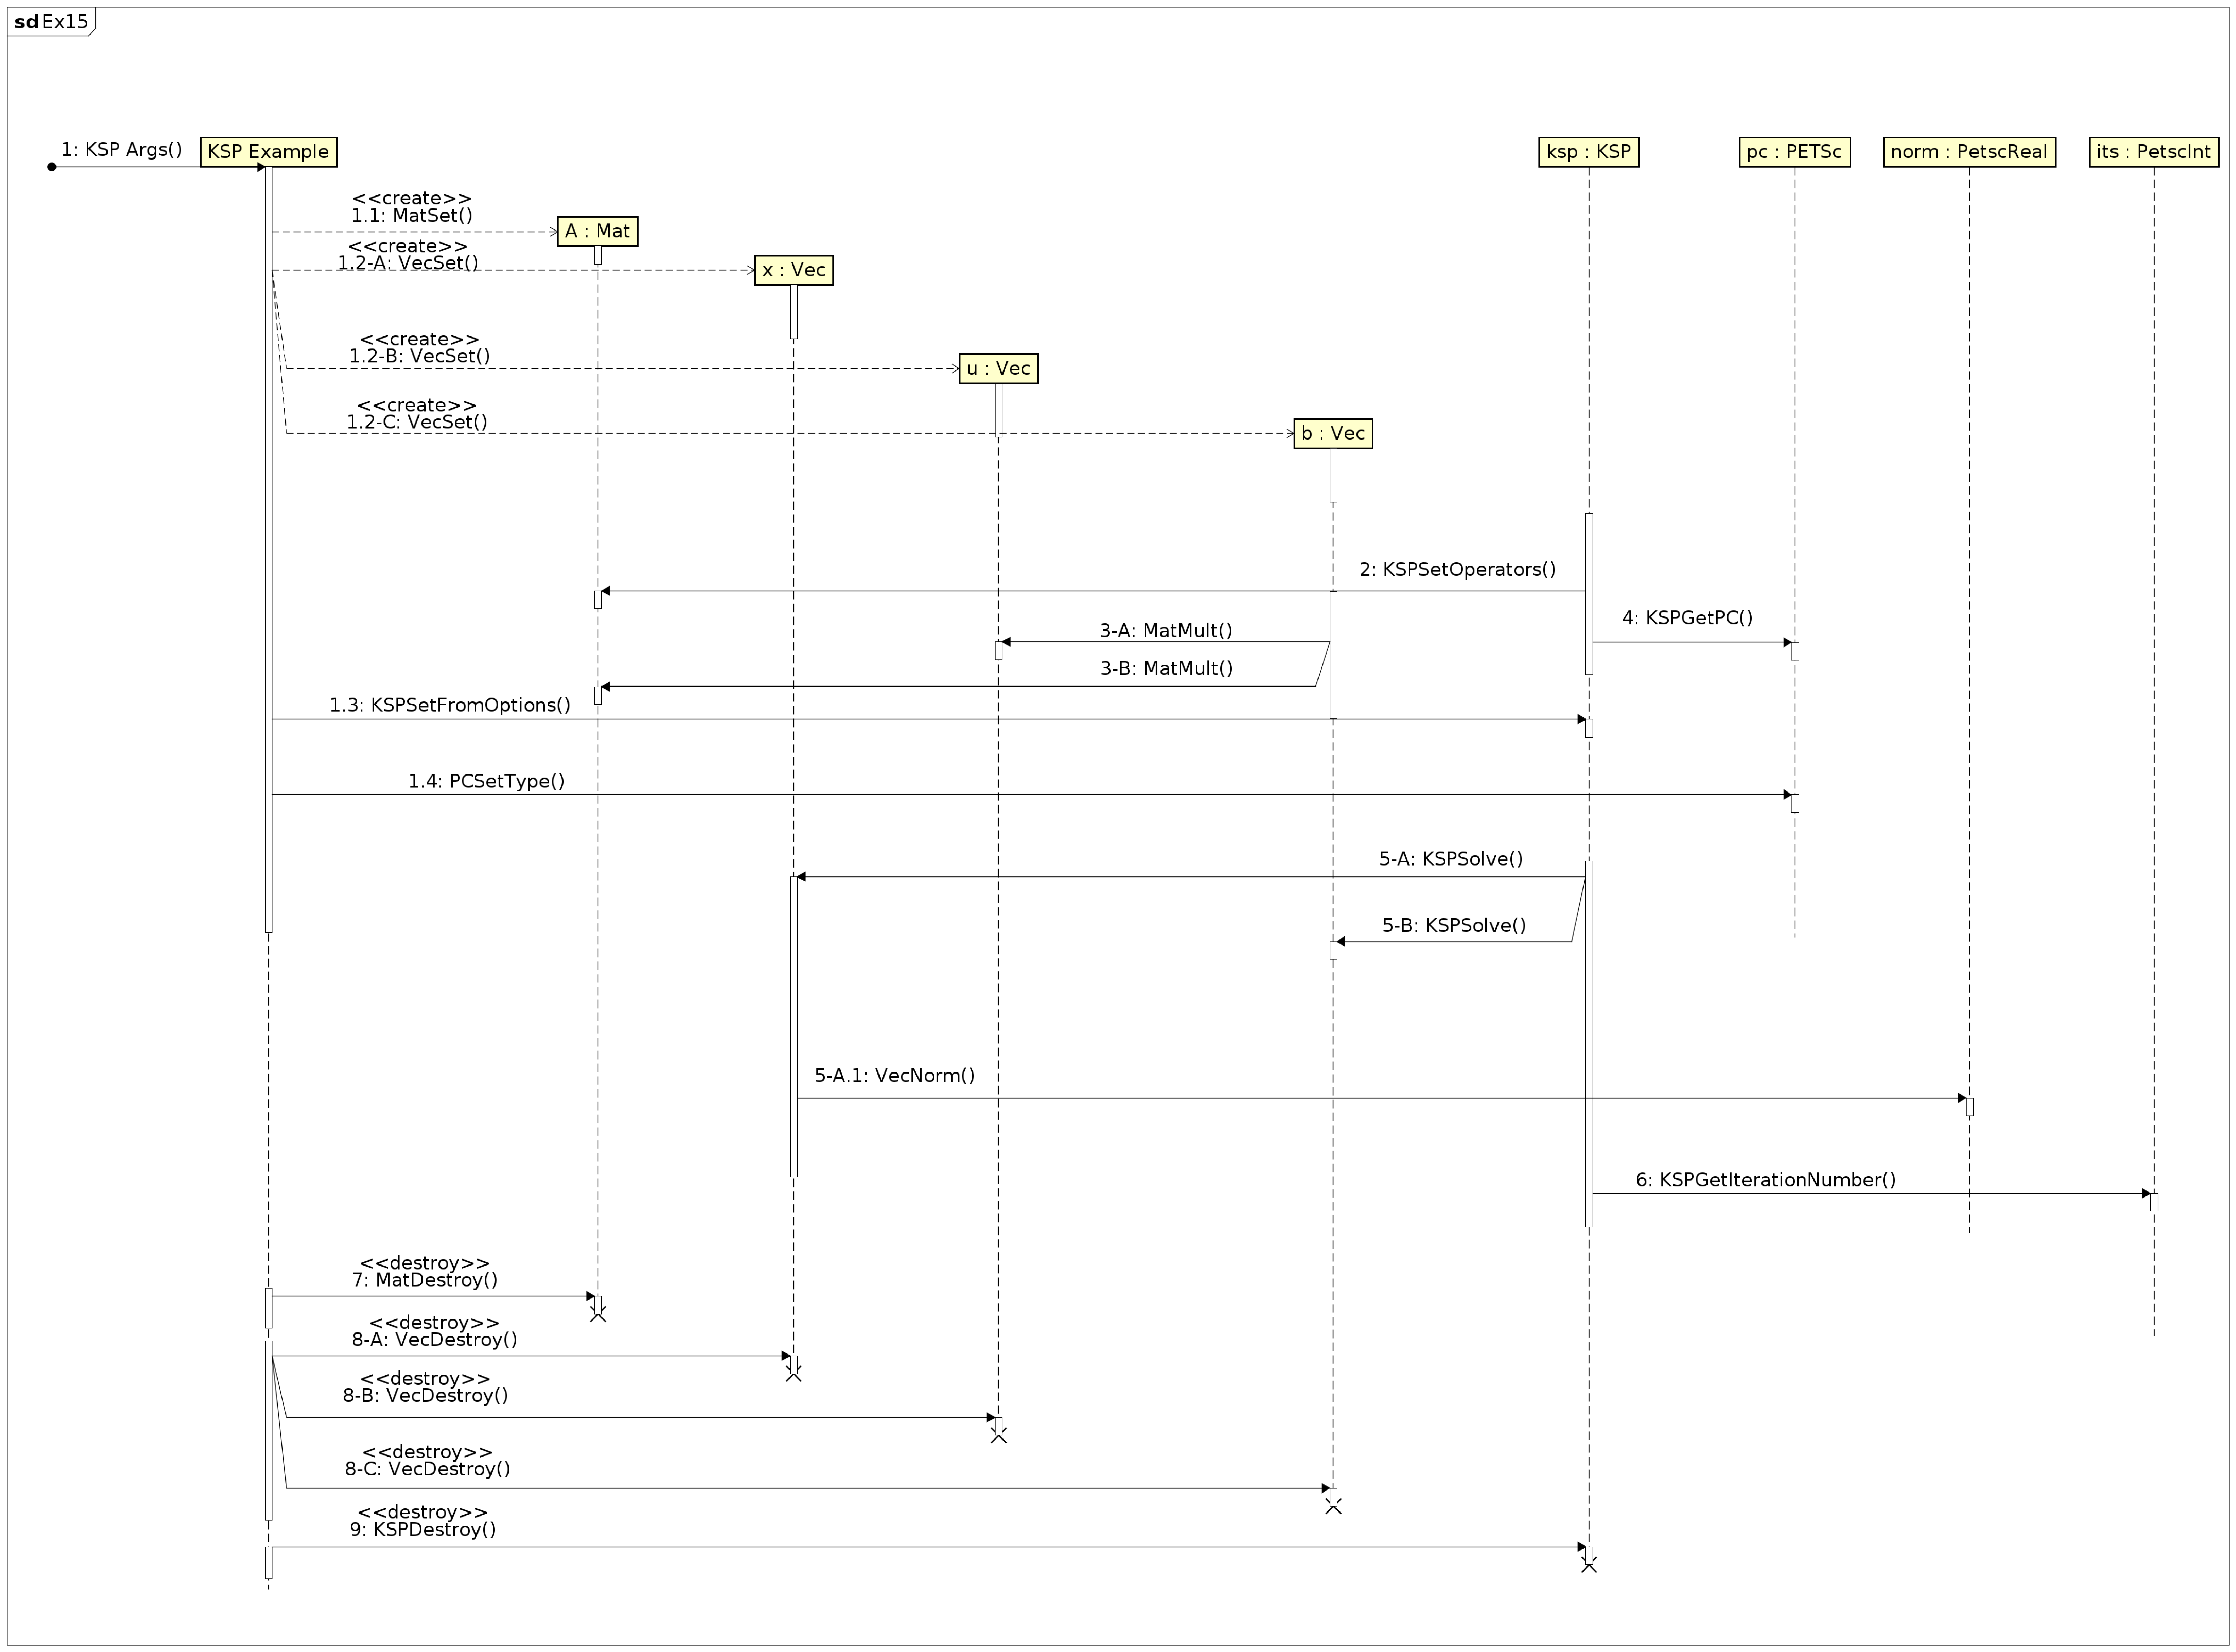
\includegraphics[width=\textwidth]{figures/Petsc_ex15.pdf}
  % \vspace{-8pt}
  \caption{Sequence diagram for PETSc Ex15}
  \label{fig:ex15}
\end{figure}



\subsection{Class Diagram for Abstract Linear Solver Factory}
For this abstract factory class diagram in \cref{fig:linalgfactory}, the abstract products consist of the objects $A$,$b$,$x$, as well as the linear function solver $LinSolve()$. These products then have variants of being either in terms of dense or sparse matrices. The abstract factory interface defines the possible products to be created, with realizations for the abstract factories for the variants (Dense and Sparse). The specific products are then dependent on these variants, for example $Sparse\_A$ is dependent on the $SparseLinearSolver Factory$. An application therefore declares specific instances of these abstract products, producing realizations of the variants of the products.
\begin{figure}[H]
  \centering
  %  trim={<left> <lower> <right> <upper>}
  % \captionsetup{skip=-12pt,format=hang}
  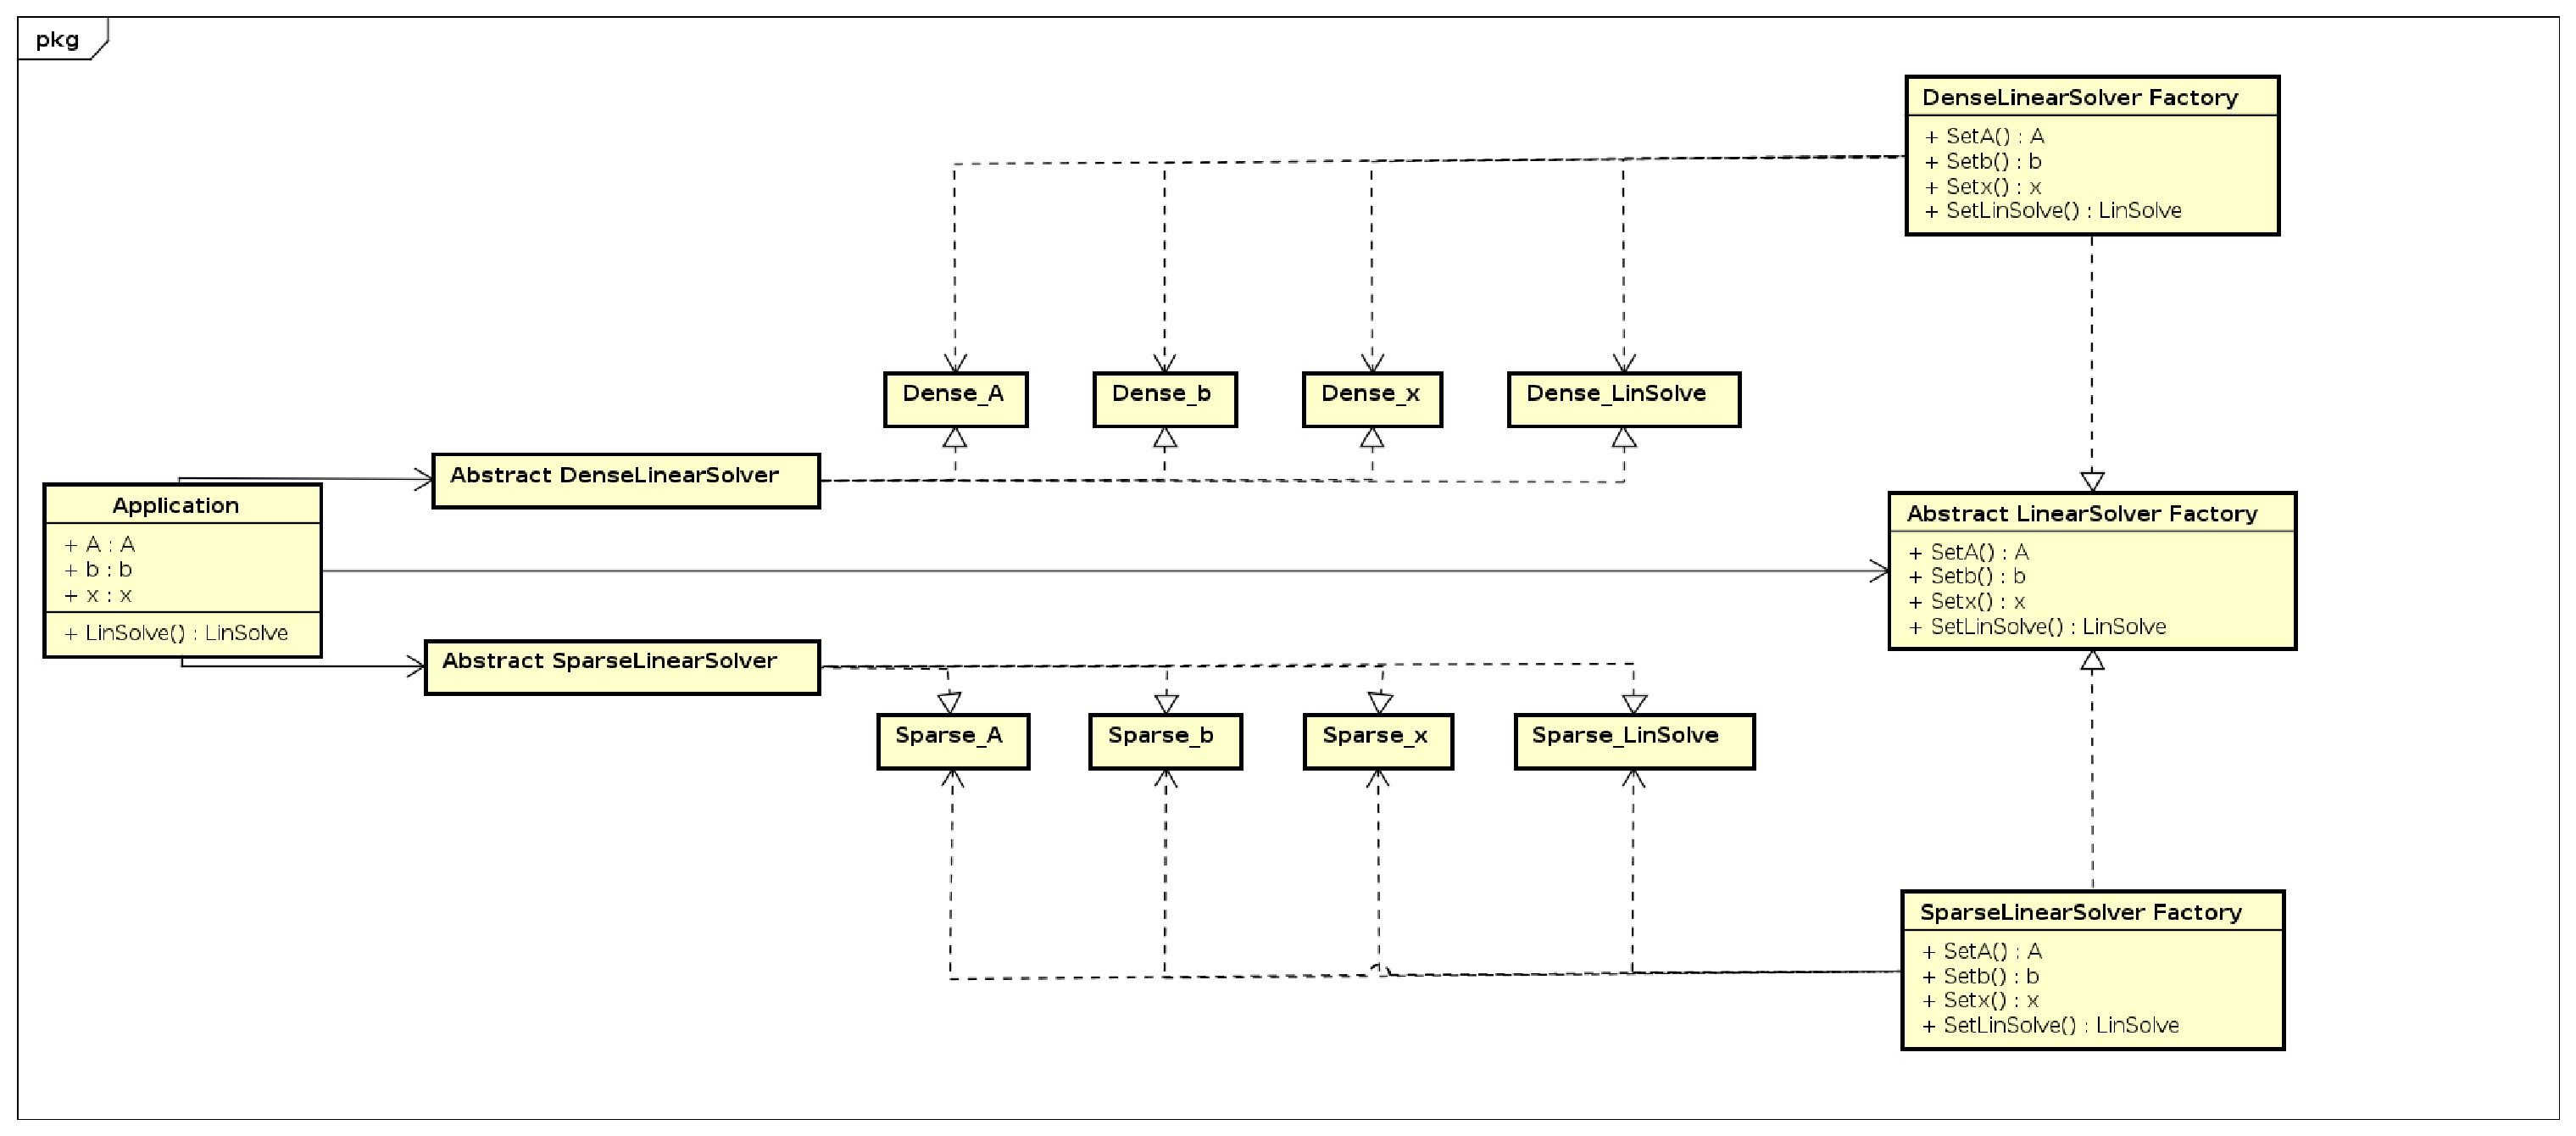
\includegraphics[width=\textwidth]{figures/LinAlg.pdf}
  % \vspace{-8pt}
  \caption{Abstract Factory Class diagram for linear solver.}
  \label{fig:linalgfactory}
\end{figure}



\subsection{Composite Class Diagram for Block Matrix}
For this composite class diagram in \cref{fig:blockmat}, the relationships between a given block matrix and its sublocks is represented by calling a $GetSublock()$ operation, which returns another recursively defined block class. There are also block operations that act on the block matrix as a whole, and return another block matrix. Each block class has a shape for rows and columns. The subblock class inherits the properties of the block class by the generalization arrow, having shape attributes and block operations on itself. The recursive, composite relation of calling sublocks and returning blocks is explained by the aggregation connection between the sublock, and the multiple nested block sublocks within it. Finally, if a sublock is composed of a single element, that element is given, and has its own element operations.
\begin{figure}[H]
  \centering
  %  trim={<left> <lower> <right> <upper>}
  % \captionsetup{skip=-12pt,format=hang}
  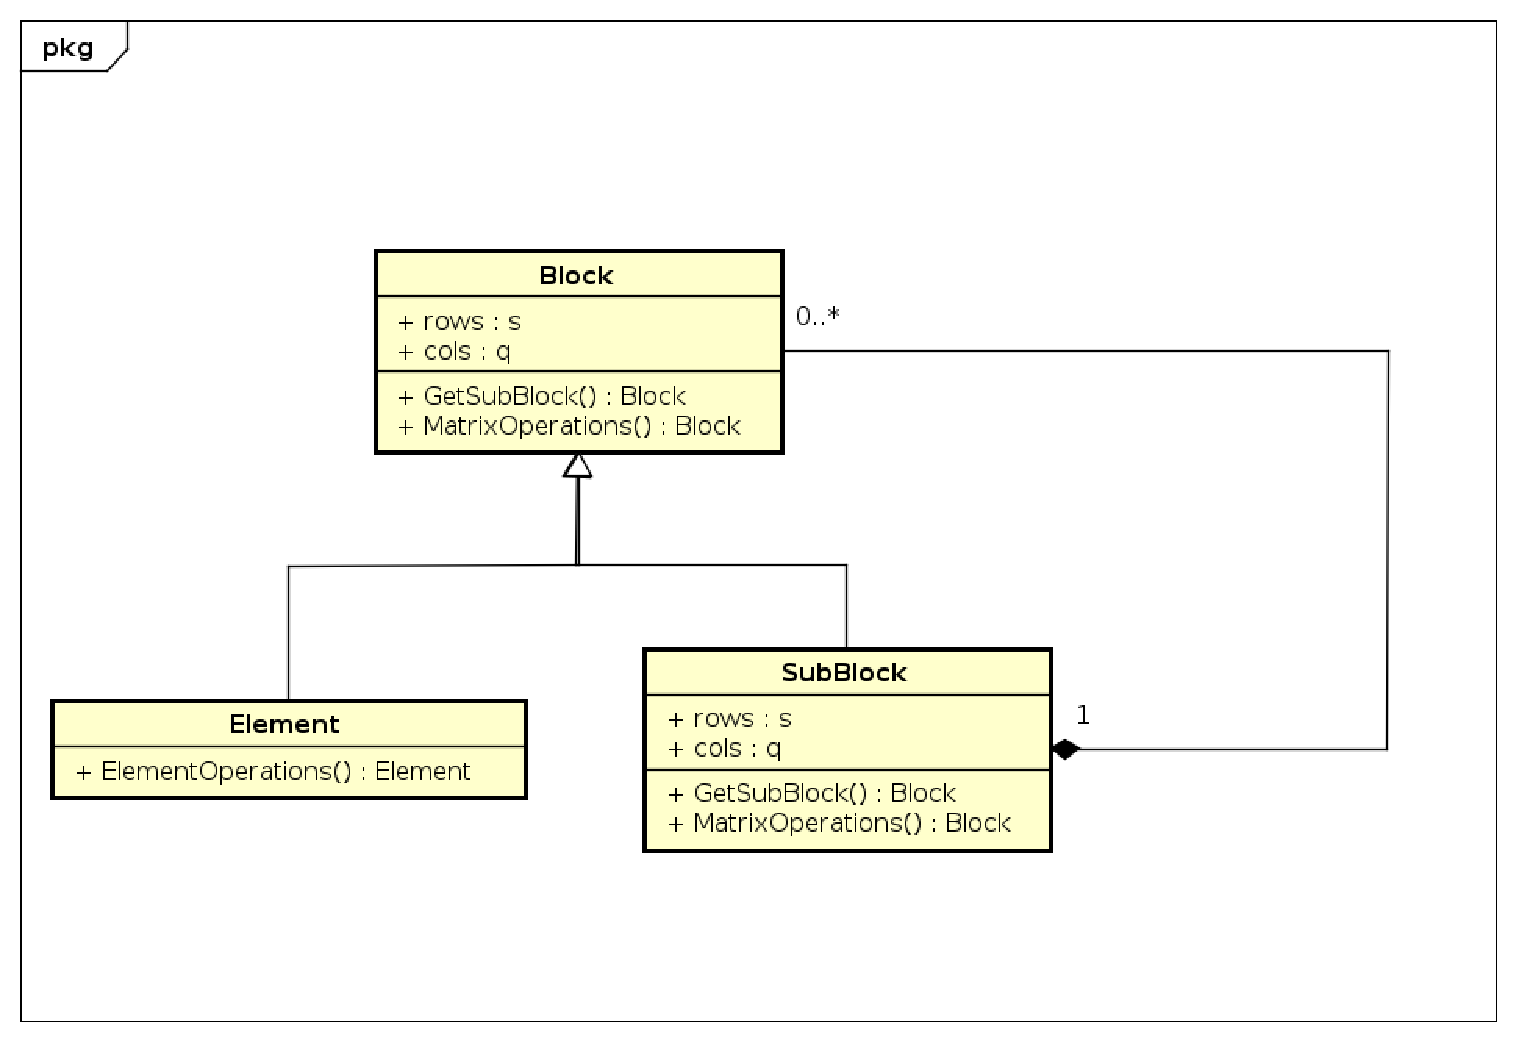
\includegraphics[width=\textwidth]{figures/BlockMatrix.pdf}
  % \vspace{-8pt}
  \caption{Composite Class diagram for block matrix.}
  \label{fig:blockmat}
\end{figure}




\newpage
\section{Sparse Matrix - Vector Multiplication Deliverables}
For the sparse matrix vector multiplication class deliverables, was assigned tasks to do with the COO sparse matrix format. Please refer to the bolded issue and pull request numbers that click-able links to the github repository.

\begin{enumerate}
  \item Implemented all COO methods. including $MatVec()$ for matrix-vector multiplication, and $assembleStorage()$ and $unAssemble()$ for assembling the matrix in the COO format based on the abstracted $setCoefficient()$ calls. \textbf{Issue \repo{issues}{29} and merged pull-request \repo{pull}{64}}.

  \item Wrote unit tests for the $CooSparseMatrix$ class, to test for the assembly procedure and matrix-vector multiplication functioning properly. \textbf{Closed \repo{issues}{20}, and merged pull-request \repo{pull}{65}}.

  \item Consulted with Eric P to fix issues in the skeleton code, and unit tests, and approved and merged the issue that Eric P implemented. \textbf{Closed Issue \repo{issues}{17}, and merged pull-request \repo{pull}{50}}.
\end{enumerate}


\newpage
\appendix
\begin{appendix}
\code{python}{figures/Ex1.py}{Fixed Iteration Methods.}{Ex1}
\code{cpp}{figures/QR.cpp}{QR algorithm class.}{QR}
\code{cpp}{figures/QR.hpp}{QR algorithm header.}{QRh}
\code{cpp}{figures/pde.cpp}{PDE algorithm class.}{PDE}
\code{make}{figures/Makefile}{Makefile.}{make}
\end{appendix}
%%%%%%%%%%%%%%%%%%%%%%%%%%%%%%%%%%%%%%%%%%%%%%%%
% \newpage
% \bibliographystyle{unsrt}
% \bibliography{mduschen_Ex1.bib}

\end{document}